\documentclass{article}

\usepackage{graphicx}
\usepackage{tikz}
\usepackage{tikzsymbols}
\usetikzlibrary{calc,patterns,shapes.geometric}
\pagestyle{empty}
\usepackage[margin=0pt]{geometry}
\geometry{papersize={14in,12in}}

\def\centerarc[#1](#2)(#3:#4:#5){\draw[#1] ($(#2)+({#5*cos(#3)},{#5*sin(#3)})$) arc (#3:#4:#5);}

\begin{document}
	\begin{figure}
		\centering
		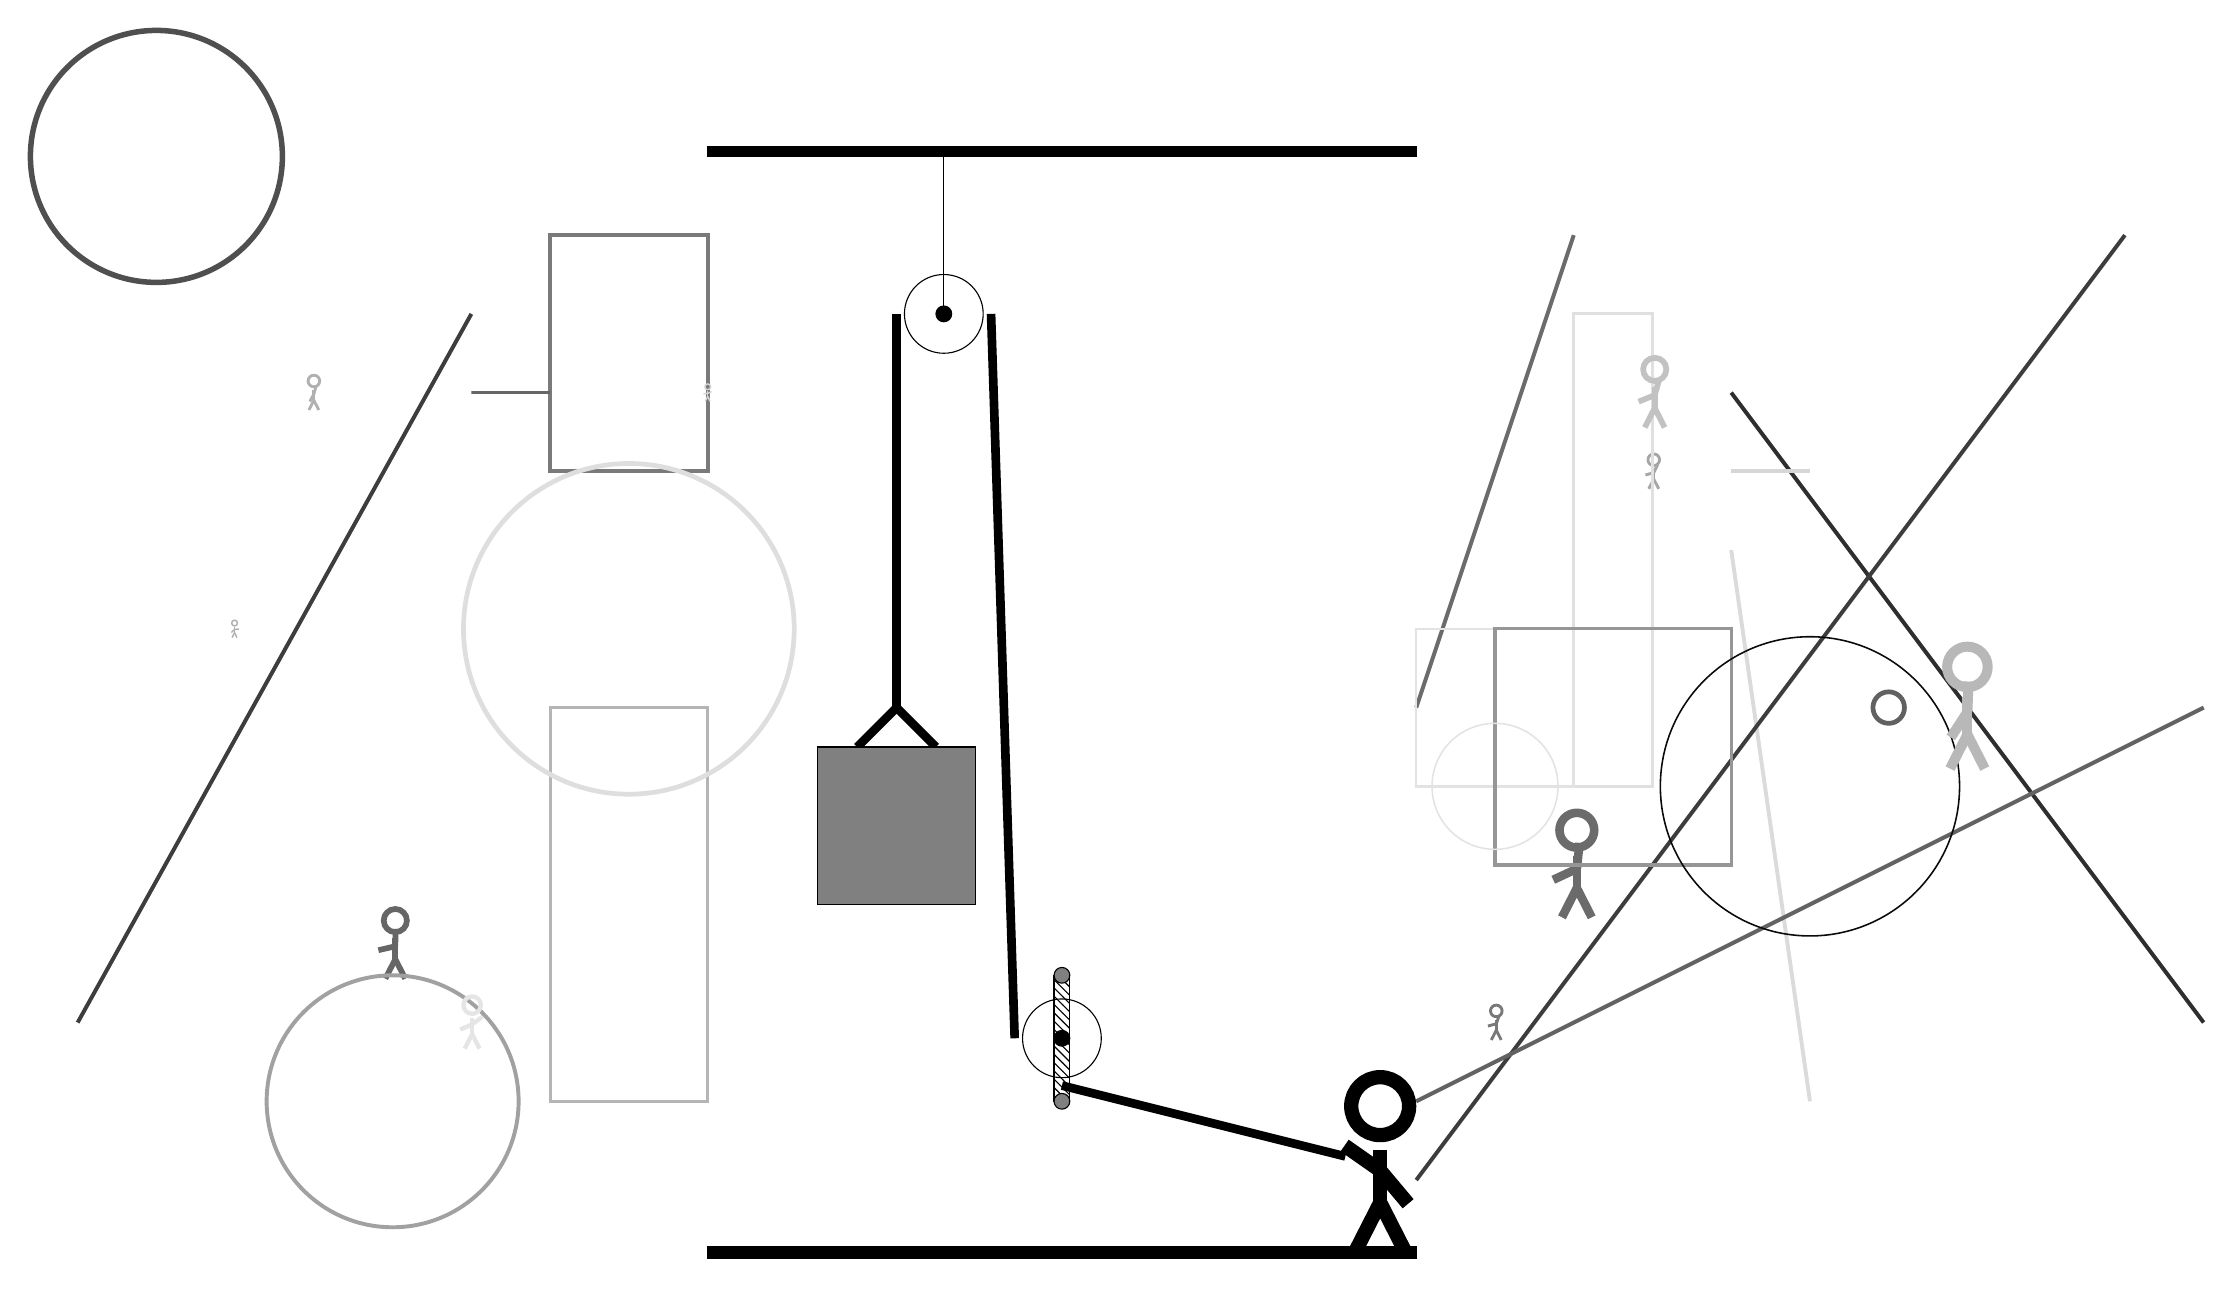
\begin{tikzpicture}
			%%%%% START %%%%%
			
			\draw[fill=black] (-2, 14) rectangle (7, 14.125);
			
			\node[line width=0.3mm, color=black!31] at (-7, 11) {\Strichmaxerl[2][62][74]};
			
			\node[line width=0.2mm, color=black!35] at (10, 10) {\Strichmaxerl[2][16][63]};
			\draw[line width=0.4mm, color=black!12] (9, 12) rectangle (10, 6);
			\node[line width=0.7mm, color=black!58] at (9, 5) {\Strichmaxerl[6][25][84]};
			\node[line width=0.3mm, color=black!24] at (10, 11) {\Strichmaxerl[4][22][74]};
			\draw[line width=0.5mm, color=black!14](12, 2) -- (11, 9);
			\node[line width=0.6mm, color=black!60] at (-6, 4) {\Strichmaxerl[4][13][89]};
			
			\draw[line width=0.5mm, color=black!58](7, 7) -- (9, 13);
			\draw[line width=0.5mm, color=black!52] (-2, 10) rectangle (-4, 13);
			
			\draw[line width=0.5mm, color=black!82](11, 11) -- (17, 3);
			
			\draw[line width=0.3mm, color=black!11] (7, 6) rectangle (9, 8);
			\node[line width=0.5mm, color=black!17] at (-2, 11) {\Strichmaxerl[1][7][22]};
			\node[line width=0.4mm, color=black!31] at (-8, 8) {\Strichmaxerl[1][44][6]};
			
			\draw [line width=0.6mm, color=black!62](13, 7) circle (0.2);
			\node[line width=0.2mm, color=black!53] at (8, 3) {\Strichmaxerl[2][15][71]};
			\draw[line width=0.5mm, color=black!16](11, 10) -- (12, 10);
			
			\draw[line width=0.4mm, color=black!29] (-2, 2) rectangle (-4, 7);
			
			\draw[line width=0.5mm, color=black!76](7, 1) -- (16, 13);
			\draw[line width=0.5mm, color=black!76](-5, 12) -- (-10, 3);
			
			\draw[line width=0.4mm, color=black!41] (8, 5) rectangle (11, 8);
			\draw[line width=0.5mm, color=black!61](7, 2) -- (17, 7);
			
			\draw [line width=0.7mm, color=black!69](-9, 14) circle (1.6);
			\draw [line width=0.5mm, color=black!37](-6, 2) circle (1.6);
			\draw [line width=0.2mm, color=black!96](12, 6) circle (1.9);
			\draw [line width=0.6mm, color=black!13](-3, 8) circle (2.1);
			\draw [line width=0.2mm, color=black!11](8, 6) circle (0.8);
			\node[line width=0.2mm, color=black!28] at (14, 7) {\Strichmaxerl[7][57][88]};
			\node[line width=0.7mm, color=black!10] at (-5, 3) {\Strichmaxerl[3][23][37]};
			
			\draw[line width=0.4mm, color=black!60] (-4, 11) rectangle (-5, 11);
			
			\draw (1, 12) circle (0.5);
			\draw[fill=black] (1, 12) circle (0.1);
			\draw (1, 14) -- (1, 12);
			
			\draw[fill=white](2.5, 2.8) circle (0.5);
			\draw[fill=black] (2.5, 2.8) circle (0.1);
			\draw[pattern=north west lines, pattern color=black] (2.4, 3.6) rectangle (2.6, 2.0);
			\draw[fill=black!50] (2.5, 3.6) circle (0.1);
			\draw[fill=black!50] (2.5, 2.0) circle (0.1);
			
			\draw[line width=1.1mm] (-0.1, 6.5) -- (0.4, 7.0) -- (0.9, 6.5);
			\draw[fill=black!50] (-0.6, 6.5) rectangle (1.4, 4.5);
			
			\draw[line width=1.1mm] (0.4, 12) -- (0.4, 7.0);
			\centerarc[line width=1.1mm](1, 12)(0:180:0.6);
			\draw[line width=1.1mm](1.6, 12) -- (1.9, 2.8);
			\centerarc[line width=1.1mm](2.5, 2.8)(180:270:0.6);
			\draw[line width=1.1mm](2.5, 2.2) -- (6.1, 1.3);
			
			\node at (6.5, 1.2) {\Strichmaxerl[10][-35][-50]};
			
			\draw[fill=black] (-2, 0) rectangle (7, 0.15);
			
			%%%%% END %%%%%
		\end{tikzpicture}
	\end{figure}	
\end{document}